\XeTeXlinebreaklocale "zh"
\XeTeXlinebreakskip = 0pt plus 1pt

\documentclass[11pt,a4paper]{article}

\usepackage{xltxtra,fontspec,xunicode}
\usepackage{amsthm, amsmath, amssymb, amsfonts}
\usepackage{abstract}
\usepackage{subcaption}
\usepackage{graphicx,float} 
\usepackage{minted}

\defaultfontfeatures{Mapping=tex-text,Scale=MatchLowercase}
\setmainfont{DejaVu Serif}
\setsansfont{DejaVu Sans}
\setmonofont{DejaVu Sans Mono}
\usepackage[slantfont,boldfont]{xeCJK} % 允许斜体和粗体
\setCJKmainfont{WenQuanYi Zen Hei}
\setCJKsansfont{WenQuanYi Zen Hei}
\setCJKmonofont{WenQuanYi Zen Hei Mono}

\usepackage{titling}

\renewcommand\refname{参考文献} 

\title{Draughts的功能及其实现}
\author{周聿浩\\ \small{2016011347}}

\begin{document}
\maketitle
\section{简介}
Draughts是一款利用Qt实现的国际跳棋游戏,支持双人在线对战。国际跳棋是十分古老的智力游戏之一,其规则是在$10 \times 10$的棋盘内,黑白双方各执20子,通过斜向移动、跳吃等手段吃掉对方更多的棋子。最终吃掉对方所有棋子或者使对方无法移动的一方获得胜利。

\begin{figure}[H]
	\centering
	\begin{subfigure}{.24\textwidth}
		\centering
		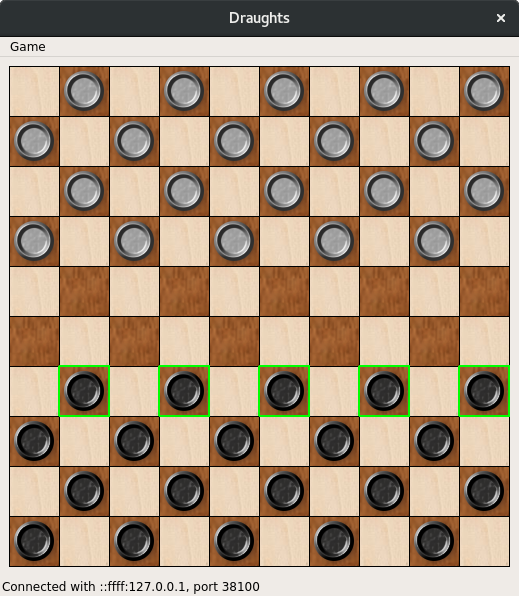
\includegraphics[width=\linewidth]{img1.png}
		\caption{}
	\end{subfigure}
	\hfill
	\begin{subfigure}{.24\textwidth}
		\centering
		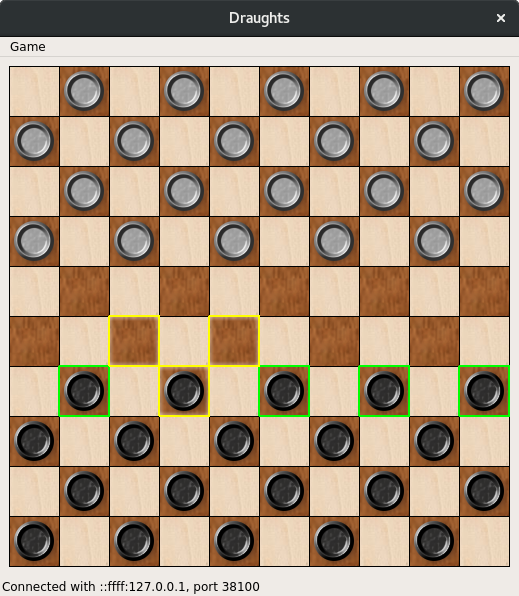
\includegraphics[width=\linewidth]{img2.png}
		\caption{}
	\end{subfigure}
	\hfill
	\begin{subfigure}{.24\textwidth}
		\centering
		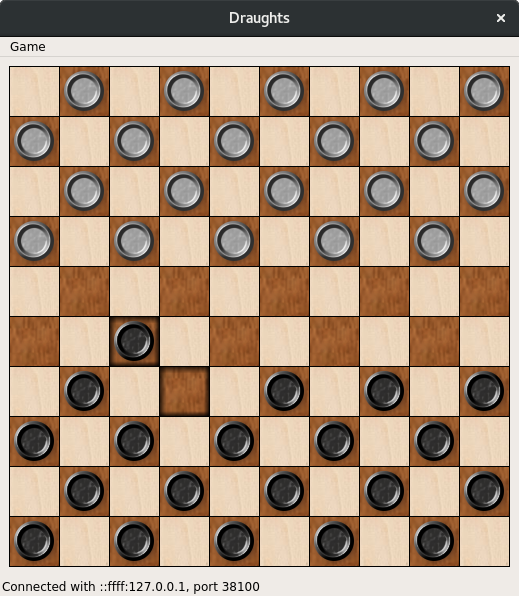
\includegraphics[width=\linewidth]{img3.png}
		\caption{}
	\end{subfigure}
	\hfill
	\begin{subfigure}{.24\textwidth}
		\centering
		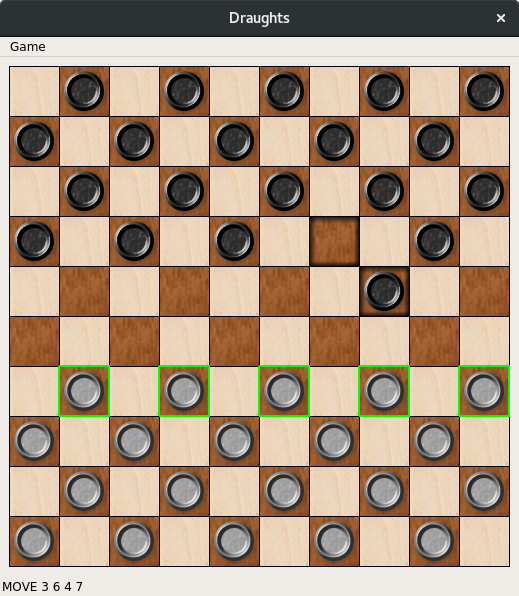
\includegraphics[width=\linewidth]{img4.png}
		\caption{}
	\end{subfigure}
	\caption{图(a):游戏开始时,黑方先手,可以移动的棋子以绿色标出。图(b):选中某个棋子后,可以移动到的空位以及当前棋子以黄色标出。图(c):移动后,移动的轨迹以黑色标出。图(d):黑方移动后,白方视角所见。}
	\label{fig:1}
\end{figure}

国际跳棋的基本规则是,黑方先行,并且所有棋子均只能斜向移动,因此整个棋盘只有深色位置可以有棋子。它有几条基本的吃子以及前进规则:

\begin{enumerate}
	\item \textbf{能吃子就必须吃}:如果有多个棋子以及多条路径都可以吃子,那么必须吃最多的棋子。如果多有条路径可以吃到相同个数的棋子,那么可以任意选择一条。
	\item \textbf{土耳其打击}:如果吃多子,那么被吃棋子在整个吃子过程结束后才被撤出棋盘。
	\item \textbf{普通棋子前进}:对于普通棋子,只能向前方对角线方向前进一格。
	\item \textbf{普通棋子跳吃}:对于普通棋子,只要对角线方向最近的黑格有敌方棋子,并且该棋子后最近的一格有空位,那么就可以跳到后方空位并且吃掉对应敌方棋子。
	\item \textbf{升王}:任何棋子在最后一步停在对方底线则称为王棋。
	\item \textbf{王棋前进}:对于王棋,只要对应方向有空位,可以向任意对角线方向前进后退任意步数。
	\item \textbf{王棋跳吃}:对于王棋,在跳吃的时候可以无时距离,并且停在被吃棋子后任意空格处。
\end{enumerate}

我们的游戏实现在当前是自己的回合时,所有可以移动的棋子会被以绿色标出。当选中某个可移动棋子时,其本身以及下一步能够移动到的位置会被以黄色标出。见图(\ref{fig:1})。

由于有连跳以及能吃子就多吃的规则,在存在多条可选路径时,如果只标明最终可达位置,可能会造成困惑以及存在无法选择相同可达位置但不同走棋路线的困难。因此,我们允许玩家一步一步进行走棋,以便选择路径,详见图(\ref{fig:2})。

\begin{figure}[H]
	\centering
	\begin{subfigure}{.24\textwidth}
		\centering
		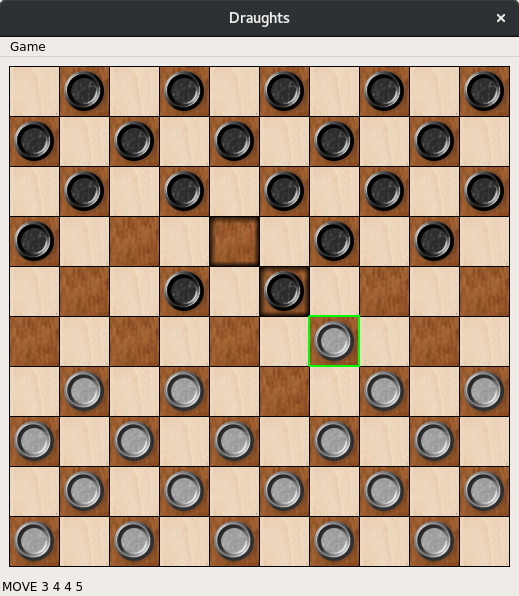
\includegraphics[width=\linewidth]{img7.png}
		\caption{}
	\end{subfigure}
	\hfill
	\begin{subfigure}{.24\textwidth}
		\centering
		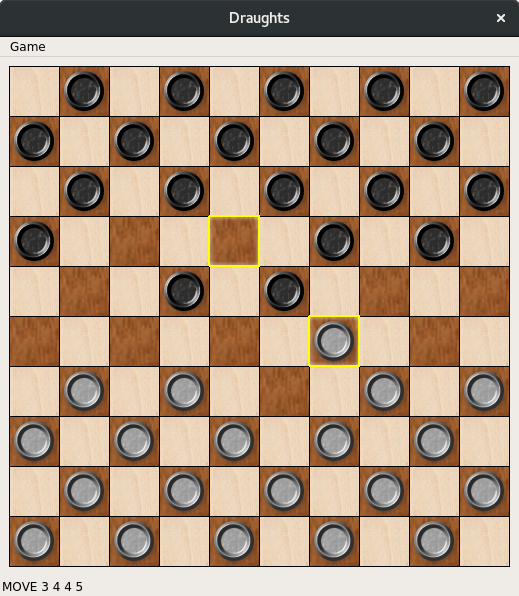
\includegraphics[width=\linewidth]{img8.png}
		\caption{}
	\end{subfigure}
	\hfill
	\begin{subfigure}{.24\textwidth}
		\centering
		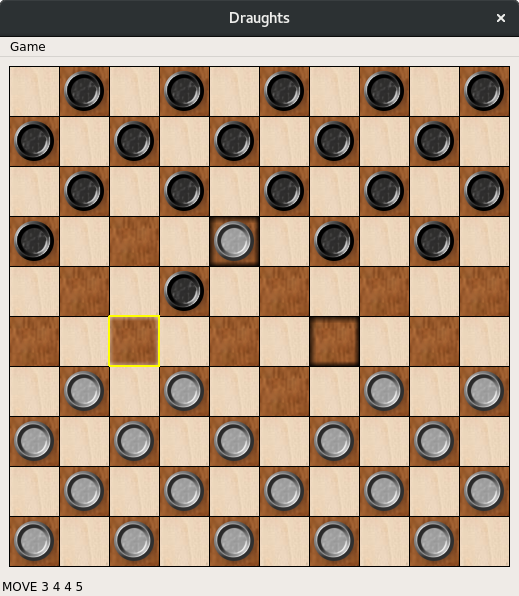
\includegraphics[width=\linewidth]{img9.png}
		\caption{}
	\end{subfigure}
	\hfill
	\begin{subfigure}{.24\textwidth}
		\centering
		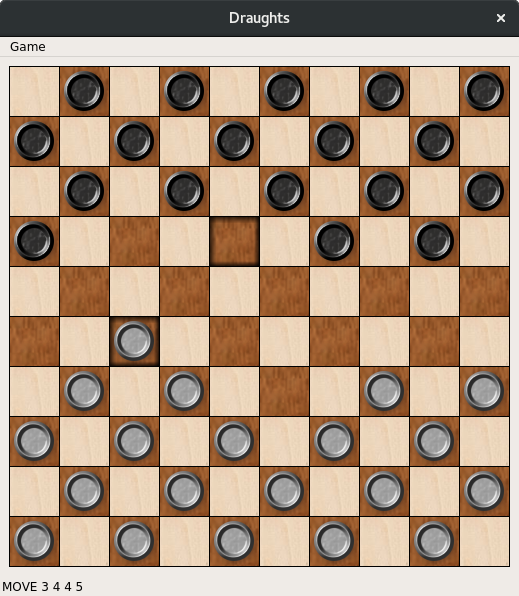
\includegraphics[width=\linewidth]{img10.png}
		\caption{}
	\end{subfigure}
	\caption{图(a):当前最多可以吃两个棋子,仅有一个棋子可选。图(b):选中后,在吃子路径的下一步被标出(如果有多条路径,全都会被黄色标出)。图(c):选择相应路径的第一步后,随即标出继续可行路径。图(d):完成一步。}
	\label{fig:2}
\end{figure}

\begin{figure}[H]
	\centering
	\begin{subfigure}{.47\textwidth}
		\centering
		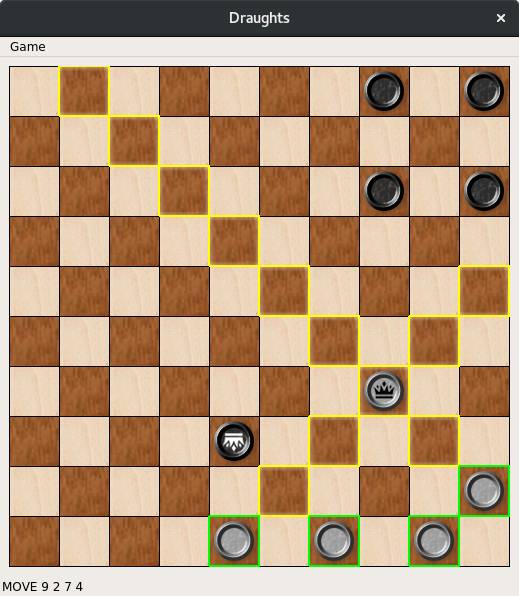
\includegraphics[width=\linewidth]{img5.png}
		\caption{}
	\end{subfigure}
	\hfill
	\begin{subfigure}{.47\textwidth}
		\centering
		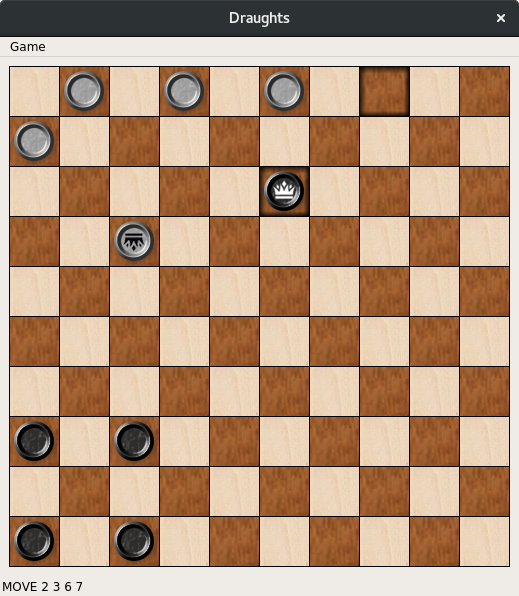
\includegraphics[width=\linewidth]{img6.png}
		\caption{}
	\end{subfigure}
	\caption{王的可行路径,以及对手所见}
	\label{fig:3}
\end{figure}

此外,在进行棋子移动时,我们提供动画效果以增加观赏性。以及增加了认输的功能(位于菜单)。

\section{部分实现细节}
关于动画效果,可以利用 {\it QPropertyAnimation} 来实现。对于被吃棋子的消失效果,可以利用 {\it QGraphicsOpacityEffect} 来调节透明度。

对于棋盘的内部黑色发光效果,可以针对矩形的四条边向内进行线性渐变的填充。

对于网络的协议,我们简单用可见字符来传输数据,以{\it 操作名+参数}的格式进行通信。例如,对于移动棋子,数据传输格式就是
\begin{center}
	MOVE {\it <length of moving trace> <pairs of (x, y)>}
\end{center}
\end{document}
